\documentclass[tikz]{standalone}
\usepackage{xcolor, amsmath, amssymb}
\usetikzlibrary{arrows.meta}
\begin{document}
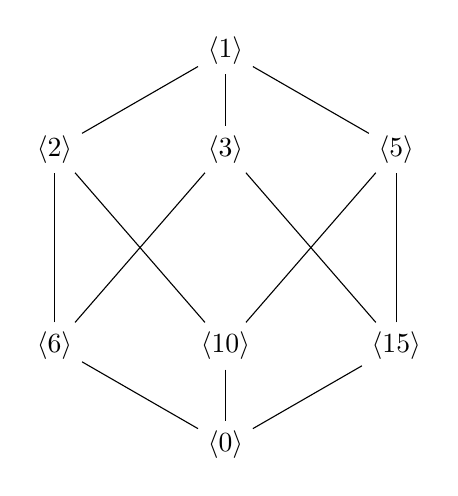
\begin{tikzpicture}
\node at(0.00, 2.50)(1){$\langle1\rangle$};
\node at(-2.17, 1.25)(2){$\langle2\rangle$};
\node at(0, 1.25)(3){$\langle3\rangle$};
\node at(2.17, 1.25)(5){$\langle5\rangle$};
\node at(-2.17, -1.25)(6){$\langle6\rangle$};
\node at(0, -1.25)(10){$\langle10\rangle$};
\node at(2.17, -1.25)(15){$\langle15\rangle$};
\node at(0.00, -2.50)(0){$\langle0\rangle$};
\draw (1) edge (2) edge (3) edge (5)
    (6) edge (2) edge (3) edge (0)
    (10) edge (2) edge (5) edge (0)
    (15) edge (3) edge (5) edge (0);
\end{tikzpicture}
\end{document}